% LaTeX template for URSI Radio Science Letters (RSL)
%
% Use pdflatex or latex + dvips + ps2pdf to produce a PDF.
%
% 15 June 2021, Henrik Wallen <henrik.wallen@aalto.fi>

%
% Submissions to RSL must use the default class option [manuscript].
% At other stages the [preprint] option can be handy.
%
\documentclass[preprint]{rsl}
%\documentclass{rsl}

%
% DO NOT add any packages or define custom macros.
%

% Title and author(s)
%
% Use explicit line-breaks \\ if needed and note that the affiliations are
% at the end of the manuscript.
%
\title{On-Body Path Loss Modeling\\ in the 110 to 170~GHz Frequency Range}
\author{Brecht De Beelde,
Reza~Aminzadeh,
Arno~Thielens,
Wout~Joseph
}

\begin{document}

\maketitle

%
% Manuscript contents begins.
%

\begin{abstract}
This letter presents empirical on-body path loss (PL) models for radio-frequency electromagnetic fields (RF-EMFs) at frequencies in the D-band. 
For the first time, PL is measured at frequencies from 110 to 170~GHz with the antennas placed at heights of 1 to 6~mm above a skin phantom, and with very small antenna separations from 1 to 19~cm.
PL is measured using a vector network analyzer (VNA)-based channel sounder with frequency extenders and using vertically and horizontally polarized horn antennas. 
The measured PL is fitted to an alpha-beta-gamma model, and wideband PL is fitted to a floating-intercept model.
Both models have a high reference PL and low PL exponent below 1. 
Even though the frequency dependence is small, PL increases with frequency. 
The measured PL is higher when the antennas are closer to the skin phantom.
\end{abstract}

\section{Introduction\label{sect:intro}}

In the last decade, the domain of personal area networks (PAN) has evolved into wireless body area networks (WBANs), where sensor and actuator nodes in and on the body wirelessly transmit data to each other \cite{Patel2010} or off the body \cite{Marinova2015}. 
Numerous channel models for WBANs at frequencies below 10~GHz are available \cite{VanRoy2010} and WBANs operational at millimeter-wave frequencies are being deployed, e.g., in the V-band at 60~GHz \cite{Chahat2013,Petrillo2014,Aminzadeh2021_tap}, and the W-band around 94 GHz \cite{Brizzi2013,Ali2022}.

On-body path loss (PL) is generally studied using three approaches: theoretically \cite{Chahat2013,Petrillo2014}, numerically \cite{Reusens2009}, and using measurements \cite{Chahat2013,Reusens2009,Aminzadeh2021_tap}. 
On-body measurements have the disadvantages that they introduce subject-to-subject variation \cite{Proesmans2022} and that it is difficult for a subject to remain immobile. 
Therefore, human-body mimicking objects, so-called phantoms, are used to stabilize and standardize these measurements \cite{Chahat2013}. 
%Apart from research on radio propagation near the body, the design of antennas for WBAN applications is an active research topic \cite{Zhang2021,Mahmood2020,Hong2016,Tak2016,Verbiest2006}.

It is envisioned that future communication systems, including sixth generation (6G) wireless networks, will be important for the realization of WBANs \cite{Cornet2022}, for example in applications such as wireless prosthetics where large data rates are required over separation distances below 20~cm \cite{Proesmans2022}.
These future communication systems may use frequencies above 100~GHz, such as the D-band with frequencies ranging from 110 to 170~GHz.
D-band channel models are available for indoor \cite{DeBeelde2021_access, Pometcu2020} and outdoor \cite{DeBeelde2022_tap,DeBeelde2022_wcl} environments. 
In this letter, we present an on-body PL model for D-band frequencies. 
For the first time, on-phantom PL measurements are performed above 100~GHz to characterize the radio channel for short-range high-data rate wireless communication in WBANs.
Compared to the existing D-band channel models, not only is the presence of the skin near the Line-of-Sight (LOS) path important but the antenna separation is limited as well. 

% The outline of this letter is as follows.
% Section~\ref{sect:method} provides the measurement setup and scenarios. 
% Section~\ref{sect:results} provides the measurement results and path loss models, and Section~\ref{sect:conclusion} concludes this letter.

\section{Methodology \label{sect:method}}

A vector network analyzer (VNA) with frequency extenders is used to perform D-band channel measurements for antenna separations up to 19~cm, with a skin phantom positioned between the antennas.
In the remainder of this letter, we will refer to on-body PL measurements when the skin phantom is present near the antennas. 
This measurement setup is presented in Fig.~\ref{fig:sounder_setup}.
\begin{figure}[tb]
\begin{center}
	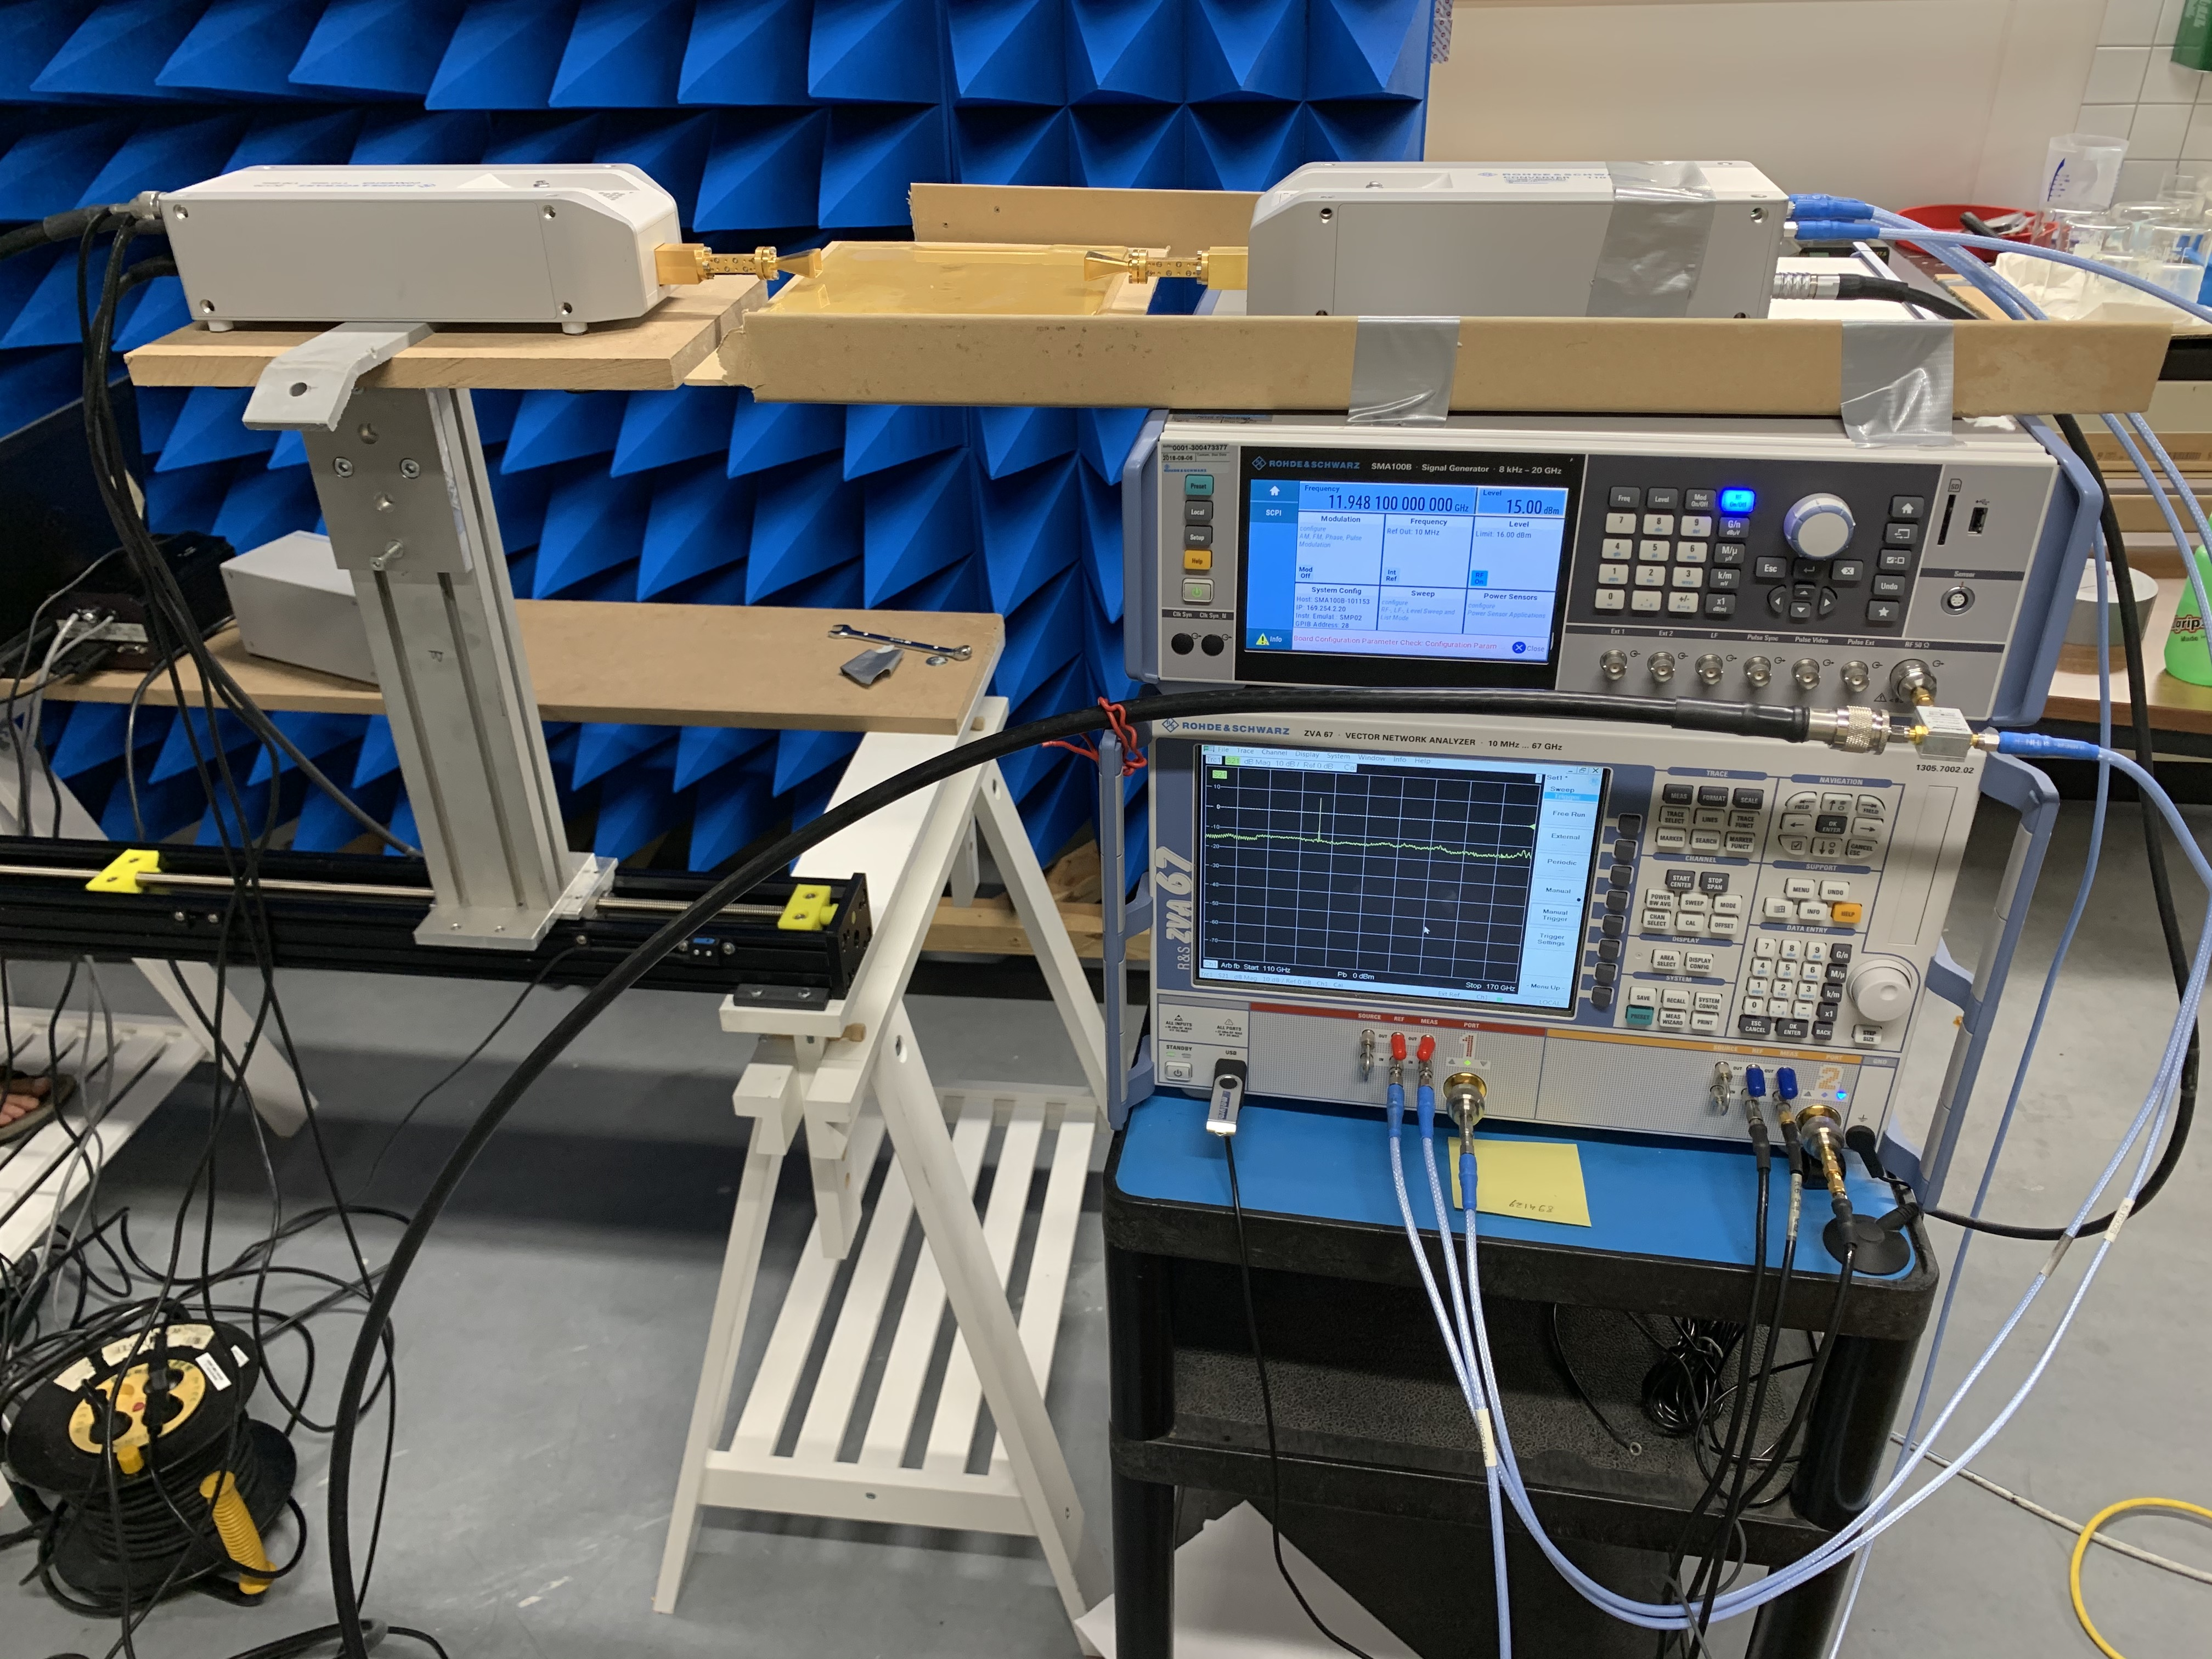
\includegraphics[width=0.45\textwidth]{figures/measurement_setup}
\caption{The measurement setup with a vector network analyzer (VNA)-based channel sounder.}
\label{fig:sounder_setup}
\end{center}
\end{figure}

\subsection{Channel sounder}

The VNA-based channel sounder that is presented and validated in \cite{DeBeelde2021_eucap} is used for the channel measurements.
%The VNA generates a radio frequency (RF) source input that is multiplied via frequency multiplication using an external frequency up-converter, which results in an RF output in the frequency range 110 to 170~GHz. 
%A harmonic mixer with a multiplication factor of 10 and a local oscillator (LO) input in the frequency range 11 to 17~GHz are used for down-conversion to generate a reference signal for the VNA. 
Quinstar standard gain pyramidal horn antennas type QWH-DPRR00 are connected to the rectangular waveguides (WR-6) of the frequency extenders. 
The antennas are operational in the D-band and have a gain increasing from 22.2~dBi for 110~GHz to 23.3~dBi for 170~GHz
The antennas have an H-plane half power beam width (HPBW) ranging from 13.2$^{\circ}$ at 110~GHz to 12$^{\circ}$ at 170~GHz and an E-plane HPBW ranging from 12$^{\circ}$ at 110~GHz to 8.8$^{\circ}$ at 170~GHz. 
The Fraunhofer far-field distance $d_F$ of these antennas, calculated via
\begin{equation}
\label{eq:Fraunhofer}
d_F = \frac{2 D^2}{\lambda}, 
\end{equation}
equals 0.55~m at 170~GHz as $D$ is equal to 0.022~m and the wavelength $\lambda$ is 0.00176~m.

A frequency sweep is performed with 3001 frequency points and a frequency step size of 20~MHz. 
The intermediate frequency (IF) measurement bandwidth (BW) of the VNA is set to 100~Hz. 
The output power is set to 16 dBm.
A normalized forward calibration is performed before all measurements, with the frequency extenders' waveguides as the reference plane of the calibration. 
No averaging is performed on the VNA, but each measurement is performed three times.
The VNA's sweep time is 45~s during which the channel is assumed to be static, as no people were moving during the measurements. 

The IF BW and transmit power settings result in a dynamic range of the sounder of 95~dB.
Due to the high bandwidth, a high temporal resolution $\Delta\tau$ of 0.0167~ns is obtained.
The maximum resolvable time delay of 50~ns corresponds to a path length of 15~m.

\subsection{Measurement scenarios}

Before the on-body measurements, reference measurements were performed and used to evaluate antenna gains, cable losses, and conversion losses over the full band \cite{DeBeelde2021_eucap}. 
The antenna separation during the reference measurements was 1.5~m, i.e., the antennas are in the far field, and no obstacles were present in between the antennas. 
%Absorbers were placed to limit the environmental influence. 

For the on-body PL measurements, the antenna separation ranged from 1~cm to 19~cm, by moving the RX antenna away from the TX antenna in steps of 3~cm.
A skin phantom was placed between the antennas. 
The antennas were placed at different heights above the skin phantom of respectively 1~mm, 3~mm, and 6~mm. 
Measurements were performed with both horizontal (HH) and vertical (VV) co-polarized antennas, by rotating the convertors by 90 degrees.

\subsection{Skin phantom}

A low-cost tissue-equivalent phantom measuring 20 by 15~cm was used to emulate the dielectric properties of a human skin. 
It has a thickness of 15~mm and is composed of 69.3\% de-ionized water, 29.7\% gelatin powder, and $\sim$1\% agar-agar~\cite{aminzadeh2014_ELetters}. 
This phantom was characterized for frequencies up to 40~GHz, but it is considered to be representative for D-band frequencies based on the following observations.
(i) In~\cite{aminzadeh2017_awpl}, a similar phantom with only 1.4\% increased mass of gelatin powder was shown to represent the skin's dielectric properties up to 100~GHz. 
(ii) In~\cite{aminzadeh2014_thesis}, an analytical model of the human skin with a water content of 70\% was validated with measurement data from literature $<$100~GHz and a maximum deviation of 10\% was reported. 
In addition, it was shown that this deviation decreased for increasing frequencies. Hence, we assume that this downward trend in error would continue in the D-band.

\subsection{Data processing}

From the measured transfer function $H(f)$, PL (in dB) is obtained via
\begin{equation}
\label{eq:PL}
\text{PL}(f)= -10 \text{log}_{10} \left( \frac{1}{N} \sum_{i=1}^N | H_i(f) |^2 \right) + 2 G_a(f) + C(f), 
\end{equation}
with $N$ the number of frequency sweeps, $G_a(f)$ the frequency-dependent antenna gain and $C(f)$ a correction term based on the reference measurements \cite{DeBeelde2021_eucap}.
After applying the Hann window $\mathcal{W}$, the inverse discrete Fourier transformation (IDFT) of the transfer function $H(f)$ results in the channel impulse response (CIR) from which the averaged power delay profile (PDP) is found. 
This is mathematically formulated as
\begin{equation}
\text{PDP}(k\Delta\tau) = \frac{1}{N} \sum_{i=1}^N | \text{IDFT}(\mathcal{W}(f) \cdot H_i(f)) |^2.
\label{eq:PDP}
\end{equation}
%The temporal resolution of the PDP $\Delta\tau$ is XX~ns, and the maximum resolvable time domain is XX~ns.
%From the PDP, the root-mean-squared (RMS) delay spread is calculated via (\ref{eq:DS}), with \dots
%\begin{equation}
%\text{PDP}(k\Delta\tau) = \dots
%\label{eq:DS}
%\end{equation}
From the PDP, wideband on-body PL is obtained. 
First, the power of the first peak of the PDP of the reference measurements (with an antenna separation of 1.5~m) is compared to free space PL (FSPL), calculated via 
\begin{equation}
\text{FSPL}(d,f)= 20 \log_{10} \left( 4 \pi d \frac{f}{\text{c}}\right), 
\label{eq:FSPL}
\end{equation}
with $d$ the distance in meters, $f$ the frequency in Hz, and c the speed of light. 
The offset (caused by antenna gains and cable losses) is then added to the power of the first peak of the PDP of the on-body PL measurements. 
This is represented via
\begin{multline}
\text{PL} = - \text{max}(\text{PDP})  + (\text{FSPL}(1.5 \text{m}, 140\cdot10^9 \text{Hz}) \\ + \text{max}(\text{PDP}_\text{ref, 1.5m}) ),
\label{eq:WB-PL}
\end{multline}
in which the first term is the peak of the PDP of the on-body measurements (positive value), and the second term is the offset between the peak the PDP of the reference measurements and FSPL.

\subsection{Path loss models}

Measured PL as a function of frequency, obtained via (\ref{eq:PL}), is fitted to the alpha-beta-gamma (ABG) model
\begin{multline}
  \text{PL}_{\text{ABG}}(d,f) = \alpha + 10 \beta \log_{10}\left(\frac{d}{\text{d}_0}\right) \\ + 10 \gamma \log_{10}\left(\frac{f}{ \text{f}_0}\right) + \chi_{\sigma},
  \label{eq:ABG}
\end{multline}
with $d$ the distance in m, d$_0$ the reference distance, $f$ the frequency in GHz, and f$_0$ the reference frequency.  
In this work, a reference distance d$_0$ of 1~cm and a reference frequency f$_0$ of 1~GHz are selected.
The model parameter $\alpha$ is the floating intercept in dB, i.e., the PL for distance d$_0$ at frequency f$_0$, $\beta$ is the dimensionless PL exponent, $\gamma$ is the dependence of PL on frequency, and $\chi_{\sigma}$ is the shadow fading term in dB \cite{Salous2020}. 

Wideband PL, obtained via (\ref{eq:WB-PL}), is fitted to the floating-intercept (FI) PL model 
\begin{equation}
  \text{PL}_{\text{FI}}(d) = \text{PL}_0 + 10 \text{n} \log_{10} (d/\text{d}_0) + \chi_\sigma, 
  \label{eq:FI}
\end{equation}
with $d$ the distance in m, d$_0$ the reference distance of 1~cm and PL exponent n. 
The shadow fading term $\chi_\sigma$ in dB is again based on a zero-mean normal distribution with standard deviation $\sigma$. 

\section{Results and discussion\label{sect:results}}

\subsection{Frequency-dependent path loss}

Figure~\ref{fig:PL_vs_freq} visualizes measured PL as a function of frequency for two polarizations and two distances, with an antenna height of 1~mm.
Fitting the measurement data to the ABG model from (\ref{eq:ABG}) results in the fitted parameters listed in Table~\ref{table:ABG}. 
Both the PL exponent $\beta$ and frequency-dependence $\gamma$ are smaller than the free space value of 2. 
The p-values of all fitted parameters are below the significance level of 10$^{-3}$. 
The error between the model and measured PL samples across all frequency and distance samples follows a normal distribution with zero mean and a standard variation close to the root-mean-squared error (RSME). 

The measured PL is higher than FSPL, and the highest PL is measured for the lowest height of 1~mm above the skin phantom.
Moreover, the measured PL for horizontal co-polarized antennas (HH) is higher than for vertically polarized antennas (VV).
The values for $\beta$ and $\gamma$ are low compared to the higher PL exponents ranging from 2 to 5 that are reported at millimeter-wave frequencies \cite{Petrillo2014, Aminzadeh2021_tap}. 
This is explained by the small antenna separations at which near-field effects need to be considered, whereas, the PL calculation in (\ref{eq:PL}) considers the far-field antenna gain.
A larger antenna inefficiency at small antenna separations results in the high measured PL values for smaller distances, which results in a smaller slope, i.e., a high reference PL ($\alpha$) and low fitted values for $\beta$ and $\gamma$.

\begin{figure}[t]
\begin{center}
  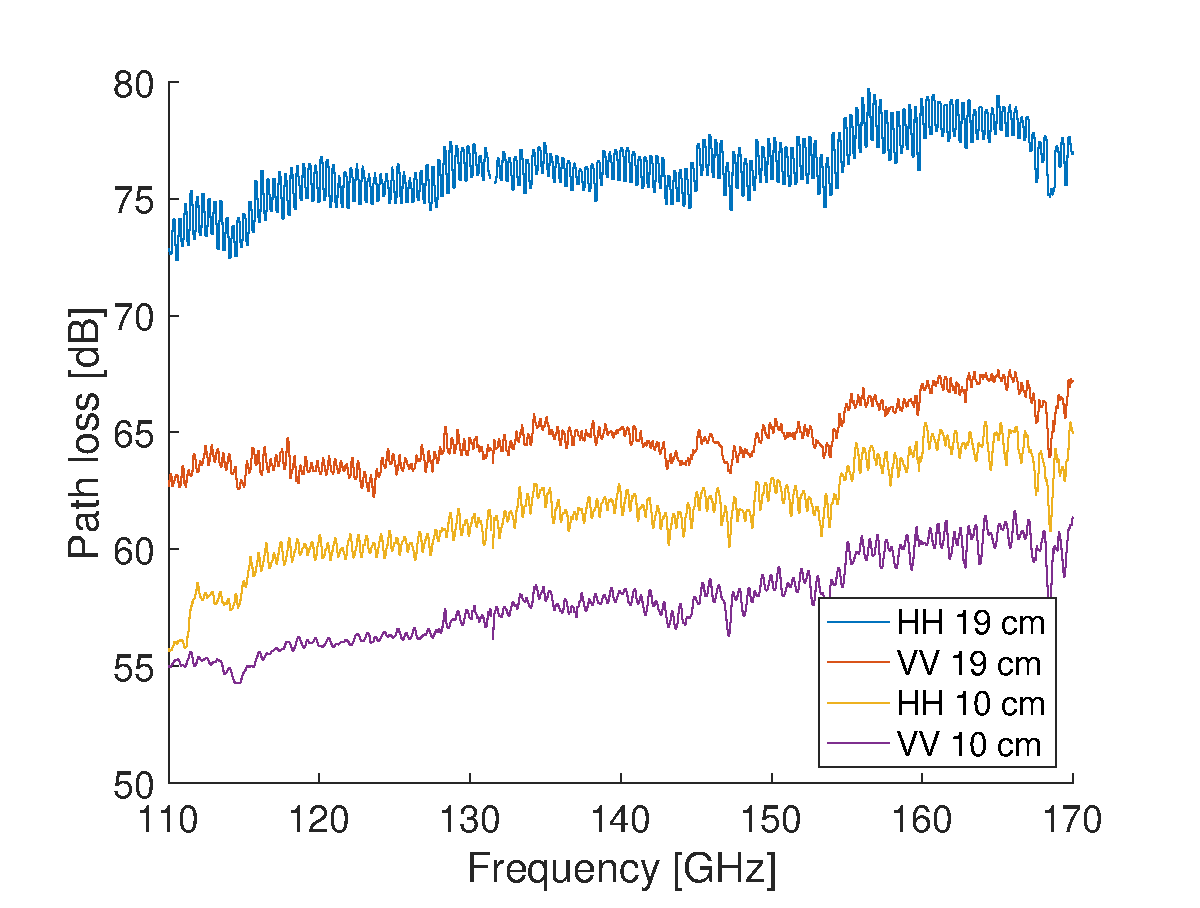
\includegraphics[width=0.45\textwidth]{figures/PL_vs_freq}
\caption{Measured path loss (PL) as a function of frequency for an antenna height of 1~mm above the skin phantom, antenna separations 10 and 19~cm, and vertical (VV) and horizontal (HH) co-polarizations.}
\label{fig:PL_vs_freq}
\end{center}
\end{figure}
\begin{table}[t]
  \caption{Fitted parameters of the ABG model for different polarizations (P) and antenna heights (H) above the skin phantom.}
  \label{table:ABG}
  \begin{center}
    \begin{tabular}{cc|cccc}
      P & H [mm] & $\alpha$ & $\beta$ & $\gamma$ & RMSE \\
      \hline
      VV & 1 & 44.6 dB & 0.54 & 0.48 & 2.7~dB \\
      VV & 3 & 38.0 dB & 0.81 & 0.62 & 3.3~dB \\
      VV & 6 & 41.2 dB & 0.65 & 0.54 & 2.6~dB \\
      HH & 1 & 26.6~dB & 3.13 & 0.30 & 3.0~dB \\
      HH & 3 & 44.5~dB & 0.68 & 0.36 & 2.3~dB \\
      HH & 6 & 45.5~dB & 0.60 & 0.34 & 2.2~dB \\
    \end{tabular}
  \end{center}
\end{table}

\subsection{Wideband path loss}

Figure~\ref{fig:PDP} shows the PDP for some select measurement scenarios. 
It is clear that round-trip reflections, i.e., reflections on the TX and RX antennas, are present.
\begin{figure}[tb]
\begin{center}
	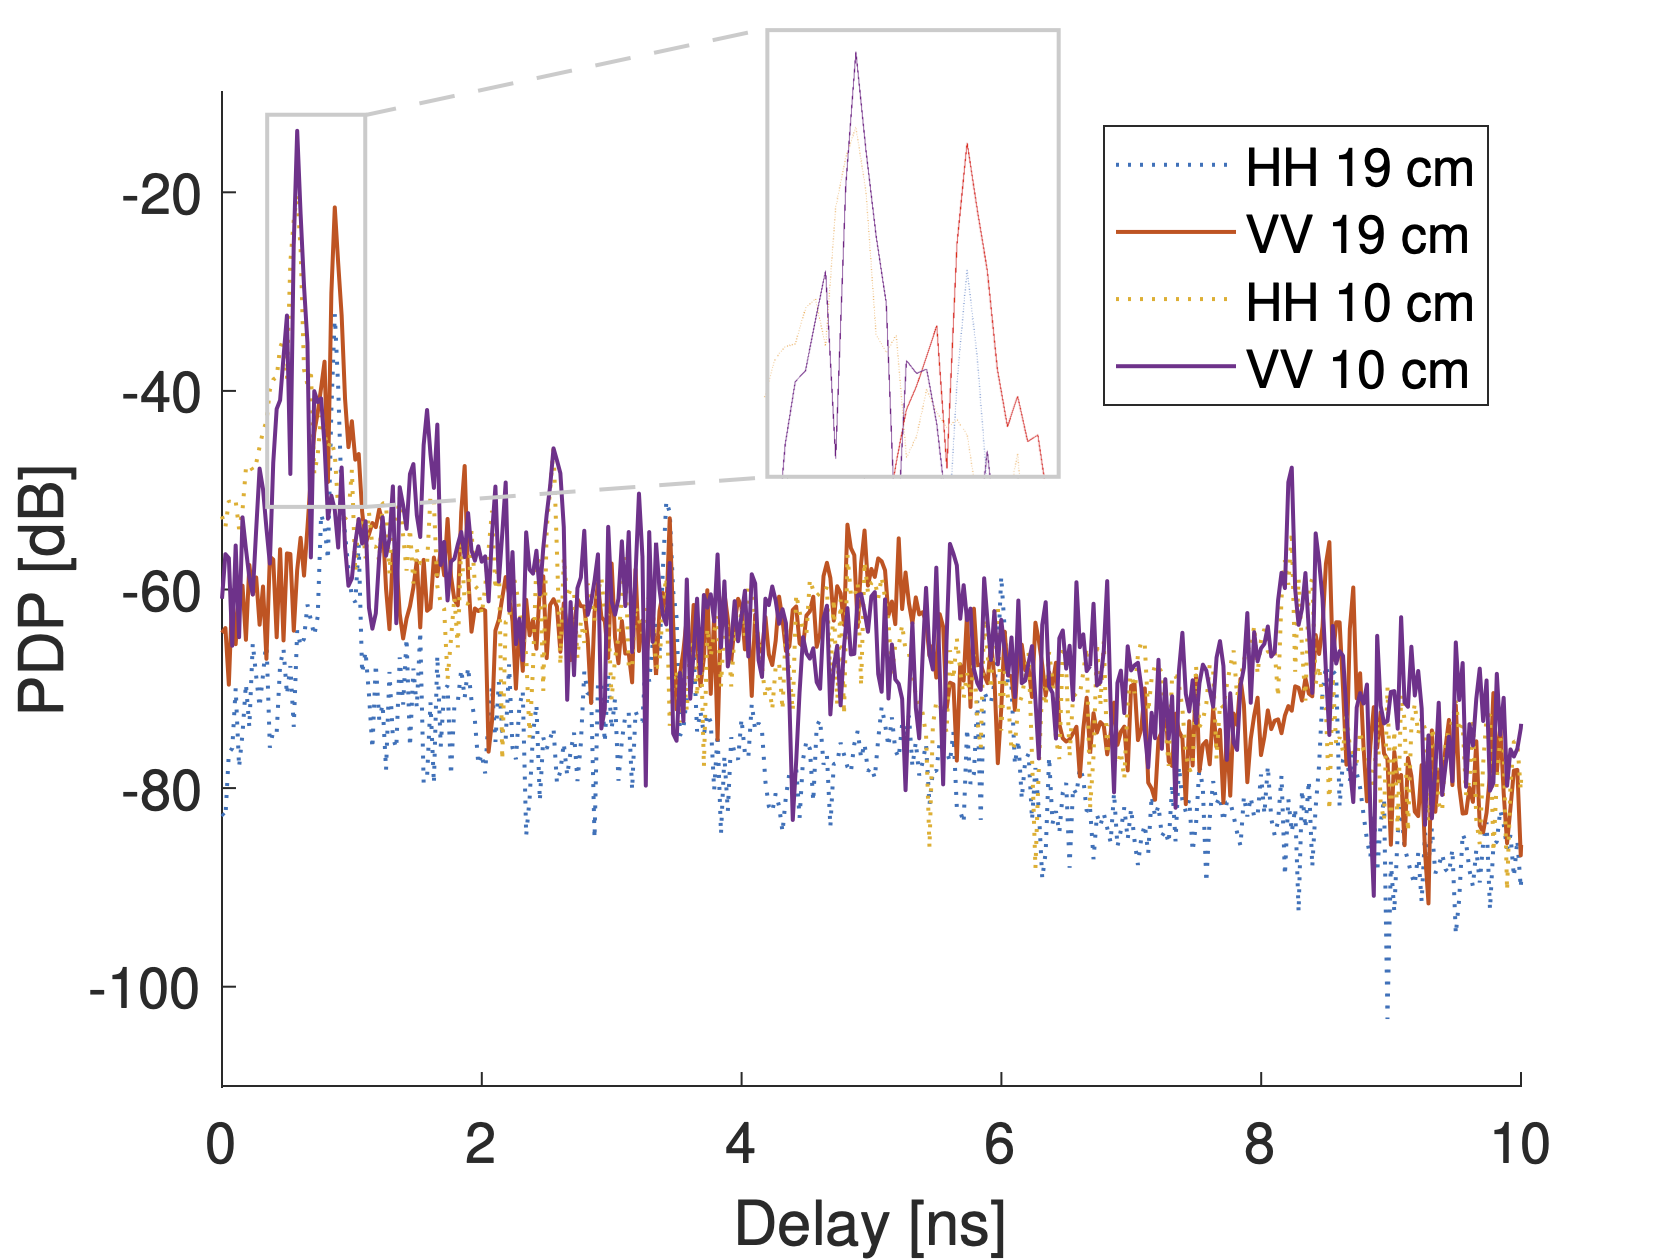
\includegraphics[width=0.45\textwidth]{figures/PDP.png}
\caption{Measured power delay profile (PDP) for different antenna separations and polarizations, with the antennas placed at 1~mm above the skin phantom.}
\label{fig:PDP}
\end{center}
\end{figure}
The reflections on the skin phantom cannot be resolved as the direct and reflected path lengths differ by less than 5~mm.

Wideband PL is obtained by selecting the power of the first peak and converting it into PL via (\ref{eq:WB-PL}). 
The measured PL as a function of distance is shown in Fig.~\ref{fig:PL_vs_dist}. 
\begin{figure}[tb]
\begin{center}
	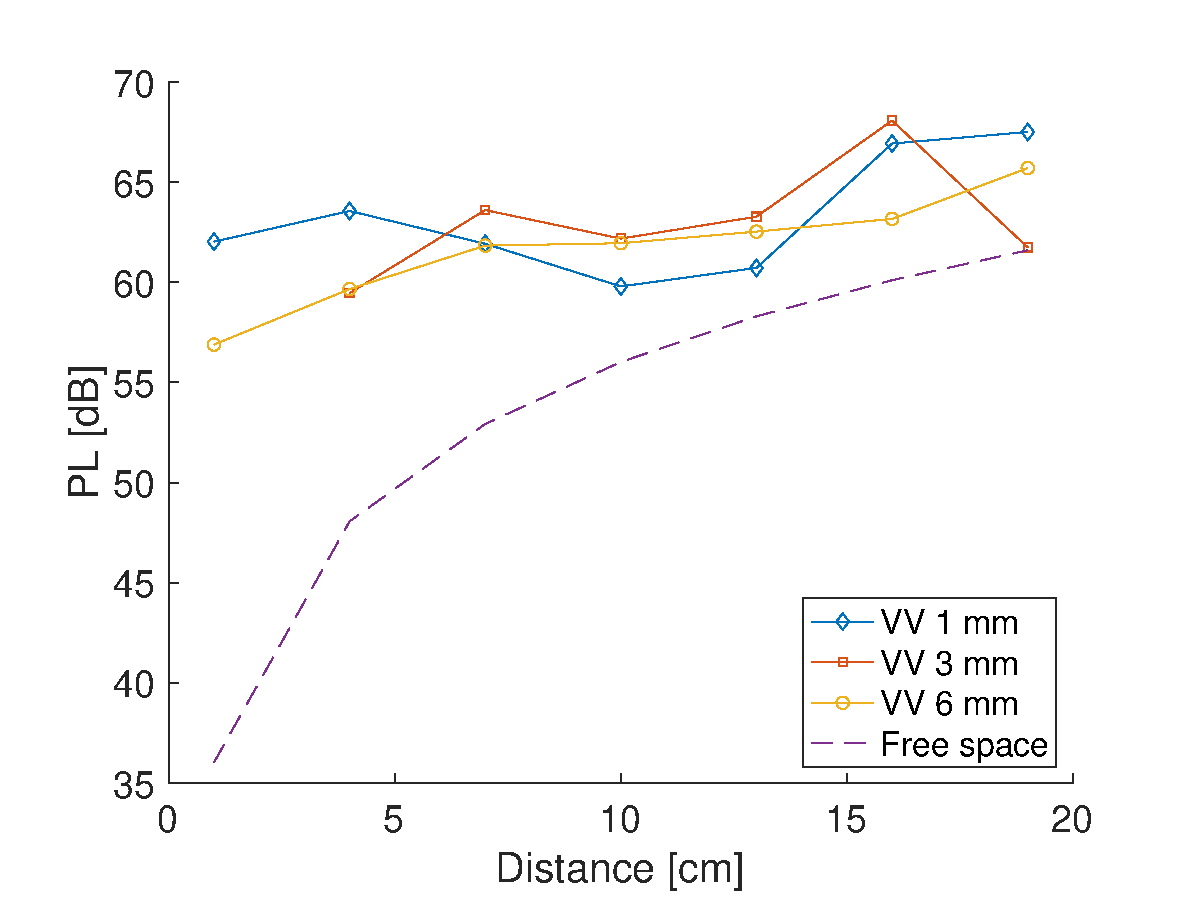
\includegraphics[width=0.45\textwidth]{figures/PL_vs_dist_VV}
	\\
	(a) VV
	\\
	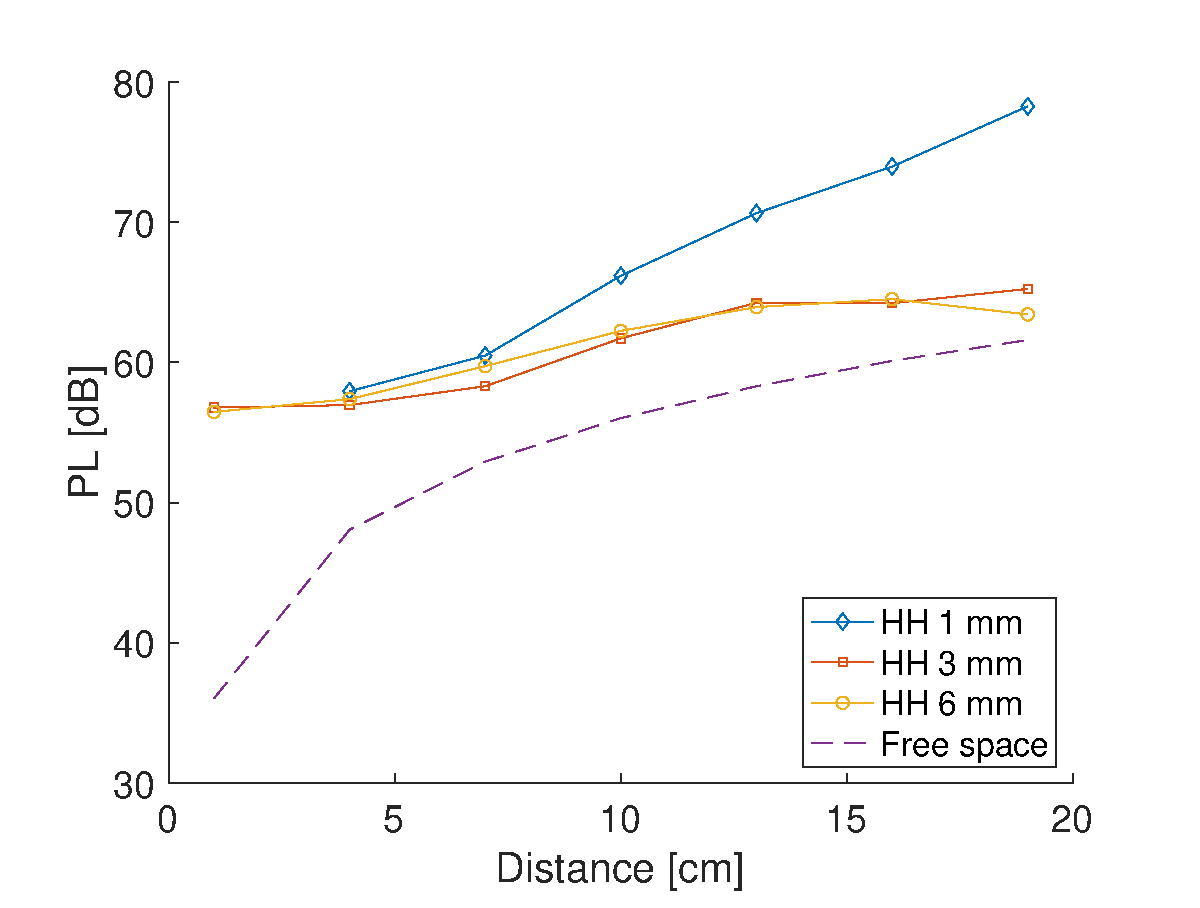
\includegraphics[width=0.45\textwidth]{figures/PL_vs_dist_HH}
	\\
	(b) HH
\caption{Measured wideband PL as a function of distance for different antenna heights.}
\label{fig:PL_vs_dist}
\end{center}
\end{figure}
From this figure, the high PL for small distances is clear, which results in the low PL exponent $\beta$ from Table~\ref{table:ABG}.
When fitting all PL samples to the FI model from (\ref{eq:FI}), similar PL exponents are obtained. 
Table~\ref{table:FI} lists the fitted parameters of the FI PL model when only antenna separations ranging from 10 to 19~cm are considered.
\begin{table}[tb]
  \caption{Fitted parameters of the FI model for different polarizations (P) and antenna heights (H) above the skin phantom for distances from 10 to 19~cm.}
  \label{table:FI}
  \begin{center}
    \begin{tabular}{cc|cccc}
      P & H [mm] & PL$_0$ & n& RMSE \\
      \hline
      % distance 1 to 19 cm
      % VV & 1 & 61.1 dB & 0.25 & 3.0~dB \\
      % VV & 3 & 56.6 dB & 0.65 & 2.6~dB \\
      % VV & 6 & 56.5 dB & 0.60 & 0.9~dB \\
      % HH & 1 & 37.3 dB & 3.04 & 2.2~dB \\
      % HH & 3 & 54.8 dB & 0.72 & 2.0~dB \\
      % HH & 6 & 55.3~dB & 0.67 & 1.4~dB \\
      % distance 10 to 19 cm
      VV & 1 & 27.7 dB & 3.14 & 1.8~dB \\
      VV & 3 & 56.6 dB & 0.65 & 2.6~dB \\
      VV & 6 & 49.2 dB & 1.23 & 0.9~dB \\
      HH & 1 & 23.5 dB & 4.24 & 0.6~dB \\
      HH & 3 & 50.5 dB & 1.17 & 0.7~dB \\
      HH & 6 & 55.3~dB & 0.67 & 1.4~dB \\
    \end{tabular}
  \end{center}
\end{table}

The difference between measured PL and FSPL is higher for small distances, due to a bad performance of the antennas, i.e., they are too close for efficient radiation. 
%Even though the antennas are still in the near field, the measured PL is closer to FSPL for larger distances. 
Due to the high PL for small distances, both the ABG and FI models result in a PL exponent well below 2, with a reference PL above FSPL. 
PL is lower when the antennas are placed at a higher height above the skin phantom. 

\section{Conclusions\label{sect:conclusion}}

In this letter, an on-body measurement campaign is presented at D-band frequencies, ranging from 110 to 170~GHz. 
The influence of distance, frequency, antenna height above the skin phantom, and polarization are investigated.
With an increased frequency, and using waveguide-based antennas, the far-field distance of the antennas increases. 
At small antenna separations, the antennas do not radiate efficiently and the boundary conditions on the phantom cause adverse propagation conditions, resulting in a high measured path loss. 
Furthermore, when the antennas are placed above a skin, the boundary conditions are unfavorable for H-polarization due to current cancelation, and the mirror effect can cause interference in the V-polarization.
Both effects result in a path loss model with a high reference path loss and low path loss exponent.
The PL is higher when the height above the phantom is lower, and for a horizontally co-polarized antenna setup. 
The latter can be caused by the larger half-power beamwidth of the antennas in the H-plane.
The PL exponent is similar to values reported in literature when only antenna separations above 10~cm are considered.
%
Future work includes analyzing the impact of different shapes of the phantom while considering LOS path blockage and antenna mismatch, e.g., caused by a wrist rotation, and a full characterization of the skin phantom at D-band frequencies. 
Furthermore, the comparison of the measurements with numerical simulations and the validation of the PL models on a real human body is pending. 
Moreover, a joint antenna and channel model where the antenna and channel characteristics are evaluated jointly would be beneficial.

\section{Acknowledgment}

This work was executed within the imec AAA D-band channel modeling research project (D-BARC). 
Arno Thielens is a postdoctoral fellow of the Research Foundation – Flanders (FWO) under grant agreement 1283921N.
\vspace{3pt}

\suppressfloats
\bibliographystyle{IEEEtran}
\bibliography{RSL_140GHz_body}
\suppressfloats

\vspace{7pt}

%
% Note that the authors' affiliations and contact information should be
% here, after the references.
%
\noindent\small
B. De Beelde, A. Thielens, and W. Joseph are with Ghent University/IMEC, Department of Information Technology, Ghent, Belgium. 
R. Aminzadeh is with Unitron Group. 
Corresponding author: B. De Beelde. 
E-mail:Brecht.DeBeelde@gmail.com
\end{document}
